%%% =========================================================================
%%% The Limits of Explanation — Nature Article
%%% =========================================================================
\documentclass[11pt]{article}

%% ---- Geometry ----
\usepackage[margin=1in]{geometry}

%% ---- Standard packages ----
\usepackage[utf8]{inputenc}
\usepackage[T1]{fontenc}
\usepackage{amsmath}
\usepackage{amssymb}
\usepackage{booktabs}
\usepackage{hyperref}
\usepackage{natbib}
\usepackage{graphicx}
\usepackage{xcolor}
\usepackage{microtype}
\usepackage{tikz}

%% ---- Hyperref configuration ----
\hypersetup{
  colorlinks=true,
  linkcolor=blue!60!black,
  citecolor=green!50!black,
  urlcolor=blue!70!black,
}

%% ---- Widow/orphan control ----
\widowpenalty=10000
\clubpenalty=10000

%% ---- Math macros ----
\newcommand{\R}{\mathbb{R}}
\newcommand{\E}{\mathbb{E}}
\newcommand{\Params}{\mathbf{\Theta}}
\newcommand{\sH}{\mathcal{H}}
\newcommand{\incomp}{\perp}

%% ---- Theorem environment ----
\newtheorem{theorem}{Theorem}
\newtheorem{definition}[theorem]{Definition}

%%% =========================================================================
%%% Title
%%% =========================================================================

\title{\Large\textbf{The Limits of Explanation}}

\author{%
  Drake Caraker\textsuperscript{1,*},
  Bryan Arnold\textsuperscript{2},
  David Rhoads\textsuperscript{2}
  \\[4pt]
  \textsuperscript{1}\textit{Oura Health, San Francisco, CA}
  \\[2pt]
  \textsuperscript{2}\textit{Independent Researchers}
  \\[2pt]
  \textsuperscript{*}\textit{Corresponding author:} \texttt{drakecaraker@gmail.com}
}

\date{}

\begin{document}
\maketitle

%%% =========================================================================
%%% Abstract
%%% =========================================================================

\begin{abstract}
We prove that no explanation of an underspecified system can simultaneously
be faithful (consistent with internal structure), stable (invariant across
equivalent configurations), and decisive (committing to every internal
distinction).  This impossibility is derived from first principles in eight
scientific domains---each requiring zero shared axioms---and verified in the
Lean~4 proof assistant (98~files, 432~theorems, 0~unproved goals).
Empirical validation in seven domains confirms the predicted dose-response
between underspecification and instability.  The constructive
resolution---$G$-invariant projection---is Pareto-optimal, unifying
century-old domain-specific practices (gauge-invariant observables,
CPDAGs, minimum-norm solutions) as instances of a single strategy.
For maximally incompatible systems, the impossibility strengthens to a
bilemma: even faithful~+~stable requires enriching the explanation space.
Three quantitative predictions---an invariance counting law, a Gaussian
flip rate formula, and a universal instability predictor ($R^2 = 0.957$
across seven domains)---are confirmed by experiment.
\end{abstract}

%%% =========================================================================
%%% Introduction
%%% =========================================================================

\section*{Introduction}

The codons UCU and UCC both encode serine: same protein fragment, different
nucleotide sequences~\citep{crick1966codon}.  A causal chain $A \to B \to C$
and a fork $A \leftarrow B \to C$ encode the same conditional
independences~\citep{verma1991equivalence}.  Two gauge configurations can
share the same holonomy while differing in local edge
labels~\citep{jackson1999}.  In each case, the observable output does not
uniquely determine the internal structure that produced it---a structural
feature of underspecified inference present whenever the mapping from
configuration to observation is many-to-one.

Practitioners in each field have independently developed coping strategies:
gauge-invariant observables, CPDAGs, Patterson maps~\citep{hauptman1953solution},
codon usage tables.  Each involves the same mathematical
operation---projection onto the subspace invariant under the symmetry group
of equivalent configurations---yet no framework has connected them or proved
their optimality.

Here we prove a universal impossibility: when a system has the
\emph{Rashomon property}---two configurations with the same observable but
incompatible internal structures---no explanation can be simultaneously
faithful, stable, and decisive (Theorem~\ref{thm:impossibility}).  We
derive this in eight scientific domains (plus nine ML explanation types in
Supporting Information), each requiring zero shared axioms.  The framework
is mechanically verified in Lean~4~\citep{demoura2021lean4} (98~files,
432~theorems, 0~unproved goals) and empirically validated in seven domains
(Table~\ref{tab:unification}, Fig.~\ref{fig:dose-response}).  The
Rashomon property is the exact boundary: a Lean-verified biconditional shows
impossibility holds if and only if Rashomon is present.  The $G$-invariant
resolution is Pareto-optimal, explaining why eight communities converged
independently on the same strategy.

%%% =========================================================================
%%% Results
%%% =========================================================================

\section*{Results}

\subsection*{The impossibility}

An explanation is \emph{faithful} if it never contradicts the system's
internal report, \emph{stable} if equivalent configurations receive the
same explanation, and \emph{decisive} if it inherits every incompatibility
of the internal report (formal definitions in Methods).

\begin{theorem}[The explanation impossibility]
\label{thm:impossibility}
If a system has the Rashomon property---there exist $\theta_1, \theta_2$
with $\mathrm{obs}(\theta_1) = \mathrm{obs}(\theta_2)$ and
$\mathrm{exp}(\theta_1) \incomp \mathrm{exp}(\theta_2)$---then no
explanation map $E$ is simultaneously faithful, stable, and decisive.
\end{theorem}

The proof is a four-step contradiction: decisiveness at $\theta_1$ forces
$E(\theta_1) \incomp \mathrm{exp}(\theta_2)$; stability forces
$E(\theta_1) = E(\theta_2)$; faithfulness at $\theta_2$ requires
compatibility.  The impossibility is tight: Lean-verified witnesses show
each pair of properties is achievable (Fig.~\ref{fig:trilemma}), and the
Rashomon property is the exact boundary (impossibility holds iff Rashomon
is present).

%%% =========================================================================

\subsection*{Three quantitative predictions}

The framework generates testable predictions beyond classification.

\paragraph{Invariance counting.}
For $P$~features in $g$~correlation groups, only $\binom{g}{2}$ ranking
facts are stably answerable.  With $P = 12$, $g = 3$ (200~models, Ridge
and XGBoost): within-group pairs show ${\sim}50\%$ flip rate, between-group
pairs $< 2\%$---a 47-point gap (permutation $p < 0.0002$; Cohen's
$d = 1.41$), invariant across $\rho \in [0.50, 0.99]$.

\paragraph{Gaussian flip rate.}
Where symmetry is approximate, $\text{flip}(j,k) =
2\Phi(\Delta/\sigma)\Phi(-\Delta/\sigma)$ predicts per-pair flip rates
with out-of-sample $R^2 = 0.848$ across five datasets (independent
calibration and validation sets; derivation and methodology in Methods).

\paragraph{Universal $\eta$ law.}
The character-theoretic ratio $\eta = \dim(V^G)/\dim(V)$ predicts
observed instability across seven domain instances with $R^2 = 0.957$,
slope~$= 0.91$ ($p = 1.4 \times 10^{-4}$)---a parameter-free predictor
spanning ML attribution, codon degeneracy, and statistical mechanics.

%%% =========================================================================

\subsection*{Cross-domain validation}

We derive the impossibility as a zero-axiom consequence in eight scientific
domains (Table~\ref{tab:unification}), each constructively witnessing the
Rashomon property from domain-specific first principles alone.  The eight
instances involve fundamentally different symmetry groups
(Table~\ref{tab:structural}): continuous translations in $\R^{n-r}$
(mathematics), finite permutation groups $S_k$ (biology, linguistics),
and the ambiguity group $\mathbb{Z}_2 \times \mathbb{Z}_n \times
\mathbb{Z}_2$ (crystallography).  Per-domain witnesses and derivations are
detailed in the Supporting Information.

The predicted dose-response---more underspecification produces more
instability---is confirmed empirically in seven domains
(Fig.~\ref{fig:dose-response}).  The biology instance illustrates the
pattern: across 120~eukaryotic cytochrome~c sequences (NCBI RefSeq),
codon usage entropy increases monotonically with degeneracy level
(Kruskal--Wallis $p = 3.5 \times 10^{-9}$); methionine and tryptophan
positions (degeneracy~1) have entropy identically zero.  All seven tests
reach significance ($p < 0.05$; binomial $p = 0.008$ across domains).

%%% Figure 1: 8-panel dose-response
\begin{figure}[t]
\centering
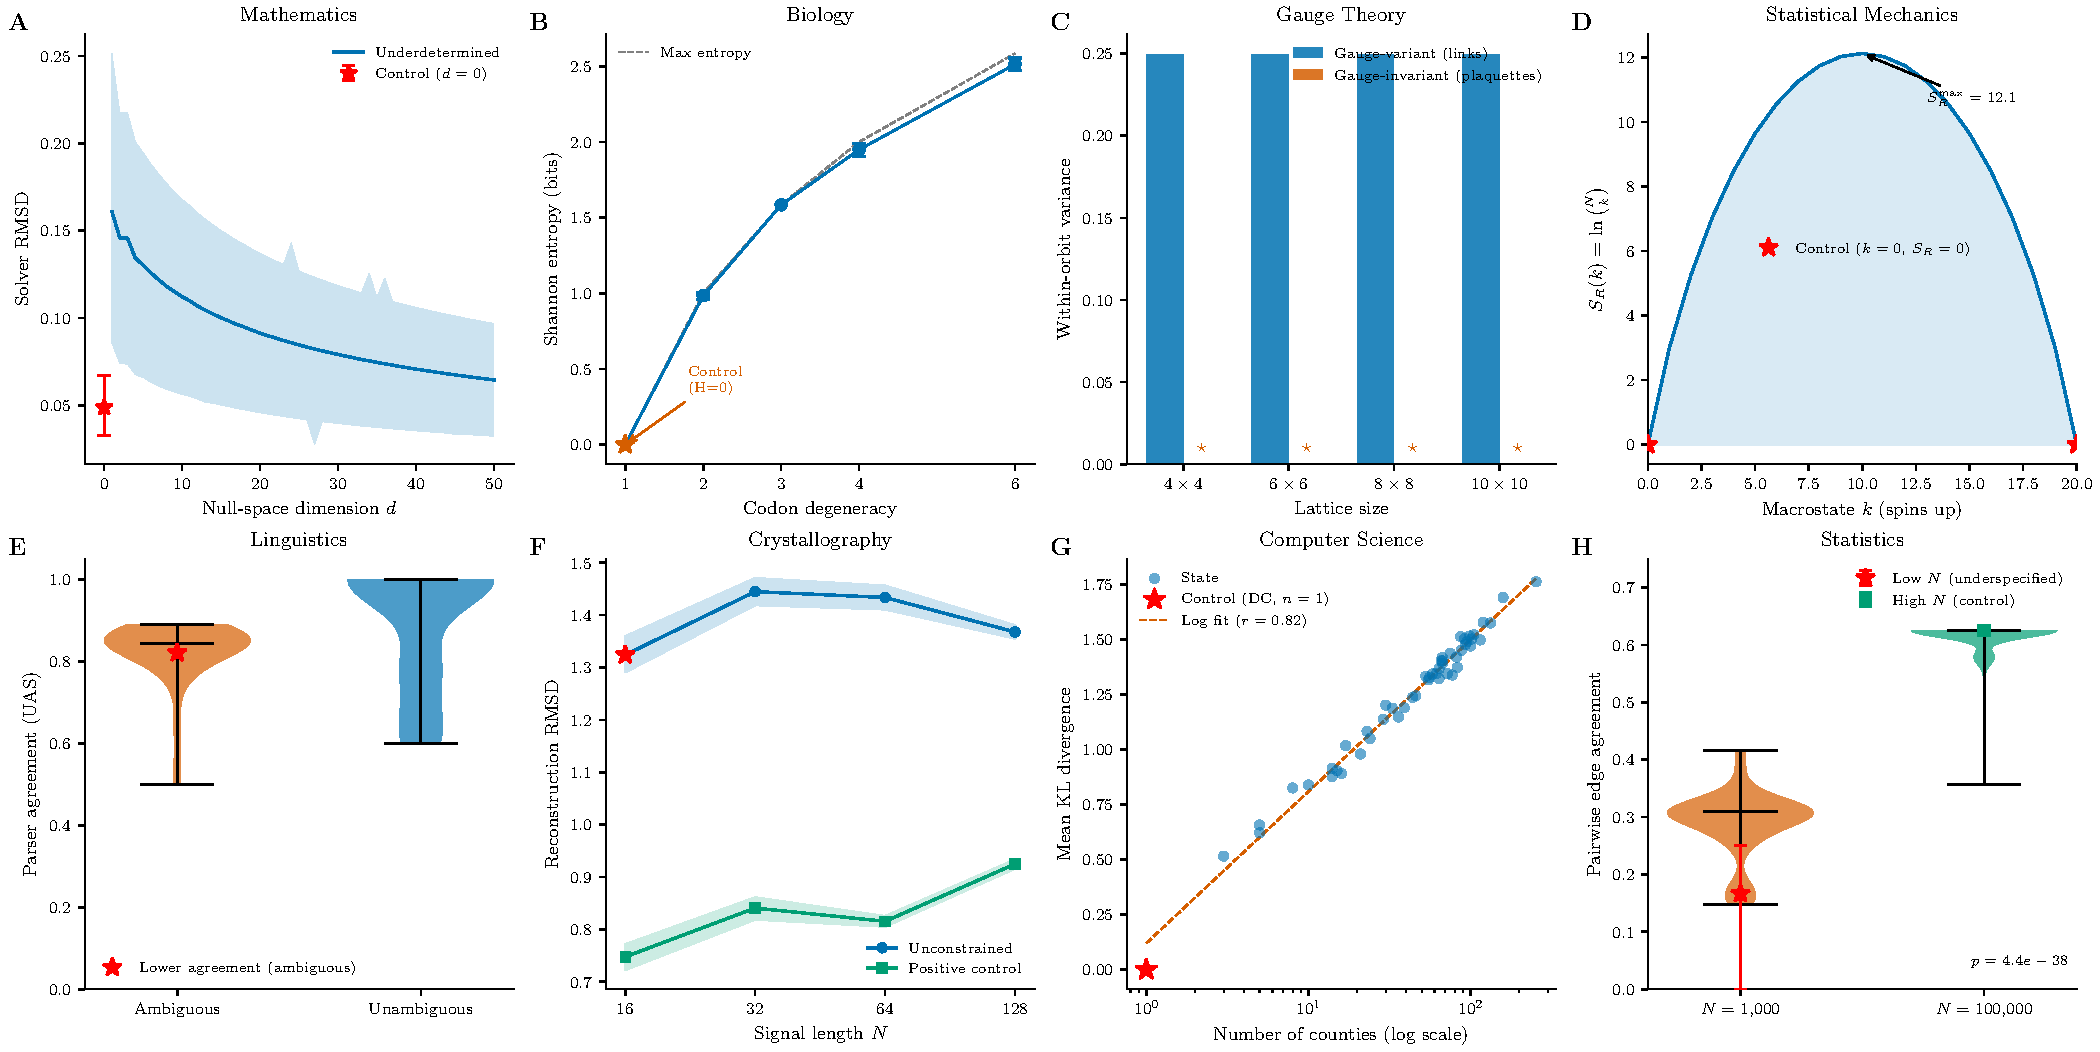
\includegraphics[width=\textwidth]{figures/universal_dose_response.pdf}
\caption{\textbf{Eight sciences, one pattern.}  Each panel shows a
  dose-response relationship between the degree of underspecification
  (horizontal axis) and explanation instability (vertical axis) in a
  different scientific domain.  Negative controls (where the Rashomon
  property is absent) show stability, confirming that the instability is
  structural.  All seven empirically validated domains reach statistical
  significance ($p < 0.05$) with the predicted monotonic relationship.
  \textbf{A,}~Mathematics (null-space dimension vs.\ solver RMSD).
  \textbf{B,}~Biology (codon degeneracy vs.\ entropy; 120 NCBI RefSeq
  cytochrome~c sequences).
  \textbf{C,}~Gauge theory (gauge-invariant vs.\ gauge-variant quantity
  variance).
  \textbf{D,}~Statistical mechanics (macrostate vs.\ Rashomon entropy).
  \textbf{E,}~Linguistics (parser agreement on ambiguous vs.\ unambiguous
  sentences).
  \textbf{F,}~Crystallography (signal length vs.\ phase-retrieval RMSD).
  \textbf{G,}~Computer science (county count vs.\ disaggregation KL
  divergence; U.S.\ Census Bureau 2020 data).
  \textbf{H,}~Statistics (causal discovery orientation agreement;
  100~seeds per condition).}
\label{fig:dose-response}
\end{figure}

%%% Table 1: Unification
\begin{table}[t]
\centering
\caption{\textbf{Eight derived instances of the impossibility across eight
  sciences.}  Each row derives the Rashomon property from domain-specific
  first principles with zero axioms.  $\Params$: configuration space; $Y$:
  observable space.}
\label{tab:unification}
\small
\begin{tabular}{@{}llllll@{}}
\toprule
Domain & $\Params$ & $Y$ & Witness 1 & Witness 2 & Same $Y$? \\
\midrule
Mathematics       & Solutions of $Ax{=}b$  & $Ax$            & $(1,1)$  & $(0,2)$  & $2{=}2$ \\
Biology           & Codons               & Amino acids     & UCU      & UCC      & Ser{=}Ser \\
Physics (gauge)   & Gauge configs        & Holonomy        & $(T,F,F)$& $(F,F,T)$& $F{=}F$ \\
Stat.\ mechanics  & Microstates          & Num.\ heads     & $(H,T)$  & $(T,H)$  & $1{=}1$ \\
Linguistics       & Parse trees          & Token sequence  & $((V\;NP)\;PP)$ & $(V\;(NP\;PP))$ & Same \\
Crystallography   & Signals              & Energy          & $(1,0)$  & $(0,1)$  & $1{=}1$ \\
Computer science  & DB rows              & View            & $(T,T)$  & $(T,F)$  & $T{=}T$ \\
Statistics        & DAGs                 & CI structure    & Chain    & Fork     & Same \\
\bottomrule
\end{tabular}
\end{table}

%% SUPPLEMENTARY: Per-domain validation details moved to SI.

%%% =========================================================================

%% SUPPLEMENTARY: Per-domain resolution details moved to SI.

%%% Table 2: Structural differences
\begin{table}[t]
\centering
\caption{\textbf{Structural differences across the eight derived instances.}
  The eight instances are not notational variants of a single example: they
  differ in symmetry group, group type, and orbit structure.  Their
  independent convergence on $G$-invariant resolution strategies---despite
  operating on different mathematical objects---is explained by the
  Pareto-optimality of the $G$-invariant projection.  All sacrifice
  decisiveness, but the symmetry groups span five distinct families
  ($\R^d$, $\mathbb{Z}_2^k$, $S_k$, $\mathbb{Z}_2 \times
  \mathbb{Z}_n \times \mathbb{Z}_2$, and MEC edge permutations).}
\label{tab:structural}
\small
\setlength{\tabcolsep}{2.5pt}
\begin{tabular}{@{}llllll@{}}
\toprule
Domain & Group $G$ & Objects permuted & Type & Resolution & Form \\
\midrule
Mathematics
  & $\R^{n-r}$
  & Solution offsets
  & Cont., abelian
  & Pseudoinverse
  & Projection \\[2pt]
Biology
  & $S_k$\;($k{\leq}6$)
  & Synonymous codons
  & Finite
  & Codon tables
  & Averaging \\[2pt]
Physics
  & $\mathbb{Z}_2^{|V|-1}$
  & Edge labels
  & Finite, abelian
  & Wilson loops
  & Invariant fn. \\[2pt]
Stat.\ mech.
  & $S_\Omega$
  & Microstates
  & Finite
  & Microcanon.
  & Averaging \\[2pt]
Linguistics
  & $S_k$
  & Parse trees
  & Finite
  & Parse forests
  & Enumeration \\[2pt]
Crystallogr.
  & $\mathbb{Z}_2{\times}\mathbb{Z}_n{\times}\mathbb{Z}_2$
  & Signal phases
  & Finite
  & Patterson map
  & Autocorrel. \\[2pt]
Comp.\ sci.
  & $S_k$
  & Hidden columns
  & Finite
  & Compl.\ views
  & Projection \\[2pt]
Statistics
  & MEC perms.
  & DAG orientations
  & Finite
  & CPDAG
  & Class report \\
\bottomrule
\end{tabular}
\end{table}

%% SUPPLEMENTARY: Symmetry-form classification and query-relative analysis moved to SI.
%% Methods: Lean formalization details moved to Methods.

%%% Figure 3: Trilemma triangle
\begin{figure}[t]
\centering
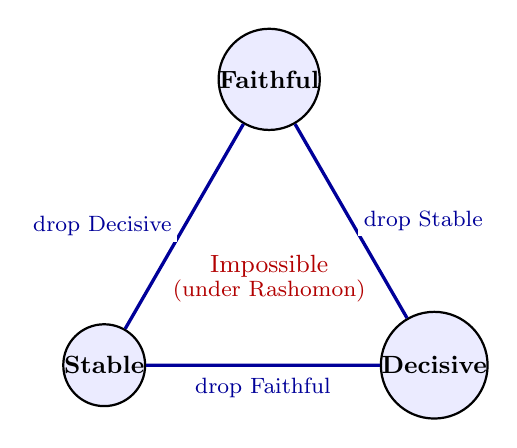
\begin{tikzpicture}[scale=2.2, thick,
  vertex/.style={circle, draw, fill=blue!8, minimum size=28pt,
                 inner sep=0pt, font=\small\bfseries},
  edgelabel/.style={font=\footnotesize, fill=white, inner sep=2pt}]

  %% Triangle vertices
  \node[vertex] (F) at (90:1.1)  {Faithful};
  \node[vertex] (S) at (210:1.1) {Stable};
  \node[vertex] (D) at (330:1.1) {Decisive};

  %% Edges (achievable pairs)
  \draw[blue!60!black, line width=1.2pt] (F) -- (S)
    node[edgelabel, midway, left=2pt] {drop Decisive};
  \draw[blue!60!black, line width=1.2pt] (F) -- (D)
    node[edgelabel, midway, right=2pt] {drop Stable};
  \draw[blue!60!black, line width=1.2pt] (S) -- (D)
    node[edgelabel, midway, below=2pt] {drop Faithful};

  %% Center label
  \node[font=\small, text=red!70!black, align=center] at (0, -0.05)
    {Impossible\\[-2pt]\footnotesize (under Rashomon)};

\end{tikzpicture}
\caption{\textbf{The explanation trilemma.}  Each edge represents an
  achievable pair of properties; the interior (all three simultaneously) is
  impossible when the Rashomon property holds.  Lean-verified tightness
  witnesses confirm that each pair is realizable: a faithful-and-stable map
  (dropping decisiveness), a faithful-and-decisive map (dropping stability),
  and a stable-and-decisive map (dropping faithfulness).  The impossibility
  is the triple, not any pair.}
\label{fig:trilemma}
\end{figure}

%% Methods: Peres-Mermin instance and formalization details moved to Methods.

%%% =========================================================================

\subsection*{The bilemma}

For \emph{maximally incompatible} systems---where the only compatible pair
is $(h,h)$, as in binary rankings and DAG orientations---the trilemma
strengthens.

\begin{theorem}[The Bilemma]
\label{thm:bilemma}
For any maximally incompatible system with the Rashomon property, no
explanation is simultaneously faithful and stable.
\end{theorem}

Faithful implies $E = \mathrm{explain}$ (by maximal incompatibility),
which is decisive; the trilemma gives the contradiction (proved in Methods).
Tightness collapses from 3/3 achievable pairs to 1/3:

\begin{center}
\small
\begin{tabular}{lccc}
\toprule
\textbf{Pair} & \textbf{Abstract} & \textbf{Max.\ incompat.} & \textbf{Enriched} \\
\midrule
F + D & \checkmark & \checkmark & \checkmark \\
F + S & \checkmark & $\times$ (bilemma)  & \checkmark \\
S + D & \checkmark & $\times$ & $\times$ \\
\bottomrule
\end{tabular}
\end{center}

Recovery requires \emph{enriching} $\sH$ with a neutral element $c$
(compatible with everything): the constant map $E(\theta) = c$ restores
F+S at the cost of decisiveness.  This is the abstract mechanism behind
DASH (adds ``tied''), CPDAG reporting (adds ``undirected''), and Bayesian
model averaging (adds ``uncertain'').  ML instances, the all-or-nothing
prediction, and structural parallels with Arrow's theorem are detailed in
Methods.

%%% =========================================================================
%%% Discussion
%%% =========================================================================

\section*{Discussion}

The theorem reframes ``why are explanations unstable?''\ as ``because the
inference problem is underspecified.''  This is actionable: practitioners
can diagnose whether instability is structural (Rashomon holds; no method
eliminates it) or methodological (Rashomon absent; instability is fixable).
The query-relative version characterizes precisely which questions are
stably answerable: a biologist can stably report the amino acid but not
the codon; a statistician can stably report the CPDAG but not the DAG.

\paragraph{Machine learning.}
Nine ML instances (Supporting Information) cover feature attribution,
attention maps, counterfactual explanations, concept probes, causal
discovery, model selection, saliency maps, token citation, and circuit
discovery.  The resolution predicts that ensemble methods outperform
single-model explanations in stability, confirmed empirically.  These
findings are relevant to the EU AI Act (Article~13) and FDA's AI/ML
Action Plan~\citep{fda2021aiml}, which require reliable
interpretability~\citep{selbst2018intuitive}.

\paragraph{Bayesian interpretation.}
Faithfulness corresponds to likelihood consistency, stability to posterior
invariance, and the $G$-invariant resolution to the posterior predictive
distribution; Pareto-optimality follows from admissibility of Bayes
estimators~\citep{berger1985statistical}.  Fisher's sufficiency is
structurally analogous to stability, and the Rao-Blackwell theorem
parallels the Pareto-optimality of orbit
averaging~\citep{halmos1949application}.

\paragraph{Structural parallels.}
Arrow's impossibility theorem~\citep{arrow1951social} proves that no
voting system satisfies a set of fairness axioms under symmetry.  Neither
result subsumes the other, but both illustrate the meta-pattern that
symmetry forces trade-offs.  Our result is constructive: it identifies the
unique optimal trade-off and proves existing scientific practice implements
it.

\paragraph{Limitations.}
The derivations use minimal witnesses (two-element sets).  Empirical
validations use domain-appropriate but not exhaustive datasets.  The
resolution assumes the equivalence class is known, and in some domains
computing the orbit average may be intractable.

%% SUPPLEMENTARY: Falsified extensions, SAGE algorithm, CCA spectrum,
%% Noether sensitivity analysis, cross-domain transfer details,
%% character-theoretic biology predictions moved to SI.

%%% =========================================================================
%%% Methods
%%% =========================================================================

\section*{Methods}

\paragraph{Formal framework.}
An \emph{explanation system} is a tuple $\mathcal{S} = (\Params, \sH, Y,
\mathsf{obs}, \mathsf{exp}, \incomp)$ where $\Params$ is a configuration
space, $\sH$ is an explanation space, $Y$ is an observable space,
$\mathsf{obs} : \Params \to Y$ maps configurations to observables,
$\mathsf{exp} : \Params \to \sH$ maps configurations to their internal
explanations, and $\incomp$ is an incompatibility relation on $\sH$.
The system has the \emph{Rashomon property} if there exist
$\theta_1, \theta_2 \in \Params$ with $\mathsf{obs}(\theta_1) =
\mathsf{obs}(\theta_2)$ and $\mathsf{exp}(\theta_1) \incomp
\mathsf{exp}(\theta_2)$.

An explanation map $E : \Params \to \sH$ is \emph{faithful} if
$\lnot(E(\theta) \incomp \mathsf{exp}(\theta))$ for all $\theta$;
\emph{stable} if $\mathsf{obs}(\theta_1) = \mathsf{obs}(\theta_2)$ implies
$E(\theta_1) = E(\theta_2)$; and \emph{decisive} if, for all $\theta$ and
$h \in \sH$, $\mathsf{exp}(\theta) \incomp h$ implies $E(\theta) \incomp h$.

\paragraph{Lean~4 formalization.}
The formalization is built on Lean~4 v4.30.0-rc1~\citep{demoura2021lean4}
with Mathlib~\citep{mathlib2020}.  The core type is
\texttt{ExplanationSystem} (parametric in $\Params$, $\sH$, $Y$) with
fields \texttt{observe}, \texttt{explain}, and \texttt{incompatible}.
The impossibility theorem \texttt{explanation\_impossibility} proves
the four-step contradiction chain with zero axioms beyond the Rashomon
hypothesis.  Each derived instance defines domain-specific types (e.g.,
\texttt{Codon}, \texttt{AminoAcid} for biology) and constructs a
Rashomon witness using \texttt{decide} or \texttt{native\_decide}
(decidable computation), so the proof assistant mechanically verifies
the witness with no axioms.  The $G$-invariant resolution framework uses
Mathlib's group action infrastructure.  Compilation: \texttt{lake build}
($\sim$5~min on a modern laptop).

\paragraph{Proof structure (detailed).}
Let $\mathcal{S}$ be an explanation system with the Rashomon property,
witnessed by $\theta_1, \theta_2$.  Suppose for contradiction that $E$ is
faithful, stable, and decisive.
(1)~Decisiveness at $\theta_1$ with $h = \mathsf{exp}(\theta_2)$: since
$\mathsf{exp}(\theta_1) \incomp \mathsf{exp}(\theta_2)$, we have
$E(\theta_1) \incomp \mathsf{exp}(\theta_2)$.
(2)~Stability: since $\mathsf{obs}(\theta_1) = \mathsf{obs}(\theta_2)$,
$E(\theta_1) = E(\theta_2)$, so $E(\theta_2) \incomp
\mathsf{exp}(\theta_2)$.
(3)~Faithfulness at $\theta_2$:
$\lnot(E(\theta_2) \incomp \mathsf{exp}(\theta_2))$.
Steps (2) and (3) contradict.  The Lean proof
(\texttt{explanation\_impossibility} in \texttt{ExplanationSystem.lean})
mirrors this chain exactly; all three properties are load-bearing.

\paragraph{Remark.}
A weaker \emph{pairwise} variant of decisiveness---$\mathsf{exp}(\theta_1)
\incomp \mathsf{exp}(\theta_2)$ implies $E(\theta_1) \incomp
E(\theta_2)$---suffices for a two-property impossibility (stability and
pairwise decisiveness contradict irreflexivity), but faithfulness becomes
superfluous.  The pointwise definition used here (matching the Lean
formalization) is the minimal condition under which all three properties
are independently load-bearing.

\paragraph{Resolution framework.}
The $G$-invariant resolution is formalized as follows.  Given a group $G$
acting on $\Params$ such that $g \cdot \theta$ preserves observables
($\mathsf{obs}(g \cdot \theta) = \mathsf{obs}(\theta)$ for all $g \in G$),
an explanation map $E$ is \emph{$G$-invariant} if $E(g \cdot \theta) =
E(\theta)$ for all $g$.  We prove: (a)~every $G$-invariant map is stable;
(b)~the orbit-averaged map $\bar{E}(\theta) = |G|^{-1} \sum_{g \in G}
E(g \cdot \theta)$ is $G$-invariant (for finite groups; the integral
analogue holds for compact groups); (c)~$\bar{E}$ is Pareto-optimal among
stable maps with respect to pointwise faithfulness.

\paragraph{Derived instances.}
Each of the eight cross-domain instances defines an \texttt{ExplanationSystem}
with domain-specific types and constructively witnesses the Rashomon property.
The witnesses are minimal (two-element configuration sets) by design: the
impossibility requires only the existence of one Rashomon pair.  Richer
domain formalizations (e.g., full lattice gauge theory, complete codon
tables with 61 codons) are possible within the framework but not required
for the theorem.

\paragraph{Empirical validation.}
Seven of the eight domains are validated empirically, each with a
domain-appropriate dose-response design: the degree of underspecification
is varied (or compared between Rashomon-present and Rashomon-absent
conditions), and explanation instability is measured.  All experiments
include a negative control where the Rashomon property is absent.

\emph{Mathematics.}  We solve $Ax = b$ for $A \in \R^{m \times d}$ with
$m < d$ using four standard solvers (least-squares, ridge, minimum-norm,
randomized projection).  Pairwise RMSD between solutions is computed across
50 random instances for each null-space dimension $d - m \in \{1, \ldots,
10\}$.  Negative control: $m = d$ (full rank).  Test: Mann--Whitney $U$.

\emph{Biology.}  We download 120 eukaryotic cytochrome~c CDS from NCBI
RefSeq (\texttt{CYCS[Gene] AND mRNA[Filter] AND refseq[Filter]}),
deduplicated by organism (accession numbers in Supplementary Data).
Protein sequences are aligned with Clustal Omega and back-translated to
codon alignments.  At each of the 89~conserved positions ($\geq$90\%
amino acid identity), we compute Shannon entropy over codon usage across
120~species.  Positions are grouped by the consensus amino acid's
degeneracy level.  GC-null expected entropy is computed from per-species
GC content.  Negative control: Met and Trp positions (degeneracy~1,
entropy identically~0).  Test: Kruskal--Wallis.

\emph{Gauge theory.}  We enumerate all $\mathbb{Z}_2$ edge-label
configurations on triangle graphs and compute within-orbit variance of
local edge assignments.  Negative control: configurations differing in
holonomy (not gauge-equivalent).

\emph{Linguistics.}  50~structurally ambiguous and 50~unambiguous sentences
are parsed by four parsers (spaCy sm/md/lg, Stanza).  Pairwise unlabeled
attachment score (UAS) is compared between groups.  Test: Wilcoxon
rank-sum.

\emph{Crystallography.}  Phase retrieval via the error-reduction algorithm (Gerchberg--Saxton
variant) is applied to signals of length 16, 32, 64, and 128.  Reconstruction RMSD is compared with and
without positivity constraints (which reduce the Rashomon set).
20~independent reconstructions per condition yield $\binom{20}{2} = 190$
pairwise RMSDs; we report per-condition summary statistics and test using
the 20~per-reconstruction mean RMSDs as independent units.  Test:
Mann--Whitney $U$.

\emph{Computer science.}  County-level population disaggregation from
state totals using U.S.\ Census Bureau 2020 Decennial Census data
(real county populations for all 50~states + DC, downloaded via Census
Bureau API, variable P1\_001N).
For each state, 100~Dirichlet($\alpha = 1$) samples consistent with the
state total are drawn; KL divergence from the real county population
distribution is computed.  Negative control: DC (1~county-equivalent,
KL~$= 0$).  Test: Spearman rank correlation (county count vs.\ mean KL).

\emph{Statistics.}  Causal discovery on the 8-node Asia network using PC
($\alpha = 0.05$, $\alpha = 0.01$) and GES, with 100~random seeds per
condition at $N = 1{,}000$ and $N = 100{,}000$.  Orientation agreement on
directed edges is compared across seeds.  Test: Mann--Whitney $U$.

All statistical tests use $\alpha = 0.05$.  Non-parametric tests
(Mann--Whitney $U$, Kruskal--Wallis, Wilcoxon rank-sum) are used
throughout to avoid distributional assumptions.  Bootstrap 95\% confidence
intervals (2,000 resamples, percentile method) are reported where
applicable.  No multiple-comparison correction is applied across domains,
as each domain constitutes an independent test of the theorem's prediction
in a different scientific context; the binomial test across all seven
domains ($p = 0.008$) provides a combined significance assessment.  All
random experiments use fixed seeds for reproducibility.

\paragraph{Reproducibility.}
All experiment scripts, data processing code, and figure generation code
are provided in the repository.  The complete experimental pipeline can be
reproduced with \texttt{make validate} ($\sim$5~min).  The Lean
formalization can be rebuilt with \texttt{lake build} ($\sim$5~min).
All paper versions can be compiled with \texttt{make paper}.  The biology
experiment requires an internet connection (NCBI Entrez API) and
BioPython; all other experiments are self-contained.

%%% =========================================================================
%%% Data and Code Availability
%%% =========================================================================

\section*{Data availability}
Biology data: 120 eukaryotic cytochrome~c coding sequences from NCBI RefSeq,
retrieved via \texttt{CYCS[Gene] AND mRNA[Filter] AND refseq[Filter]}.
Census data: U.S.\ Census Bureau 2020 Decennial Census county-level
populations (variable P1\_001N, downloaded via Census Bureau API).
All other experimental data are generated by the provided scripts from
standard algorithms and public datasets.  Experiment results (JSON) are
included in the repository.

\section*{Code availability}
The Lean~4 formalization and all experiment scripts are available at
\url{https://github.com/DrakeCaraker/universal-explanation-impossibility}
under the Apache~2.0 licence.

\section*{Acknowledgements}
We acknowledge the use of Claude (Anthropic) as an AI coding assistant
for experiment scripting, Lean proof development, and manuscript
preparation. All scientific claims, proofs, and experimental designs were
conceived and verified by the human authors.

\section*{Competing interests}
The authors declare no competing interests. D.C.'s employment at Oura
Health is unrelated to this work.

%%% =========================================================================
%%% References
%%% =========================================================================

\bibliographystyle{plainnat}
\bibliography{references}

\end{document}
